\title{Tensorboard}

\subsection{Tensorboard}

TensorBoard provides a suite of visualization tools to make it easier
to understand, debug, and optimize Edward programs. You can use it
``to visualize your TensorFlow graph, plot quantitative metrics about
the execution of your graph, and show additional data like images that
pass through it''
(\href{https://www.tensorflow.org/get_started/summaries_and_tensorboard}
{tensorflow.org}).

A Jupyter notebook version of this tutorial is available
\href{http://nbviewer.jupyter.org/github/blei-lab/edward/blob/master/notebooks/tensorboard.ipynb}{here}.

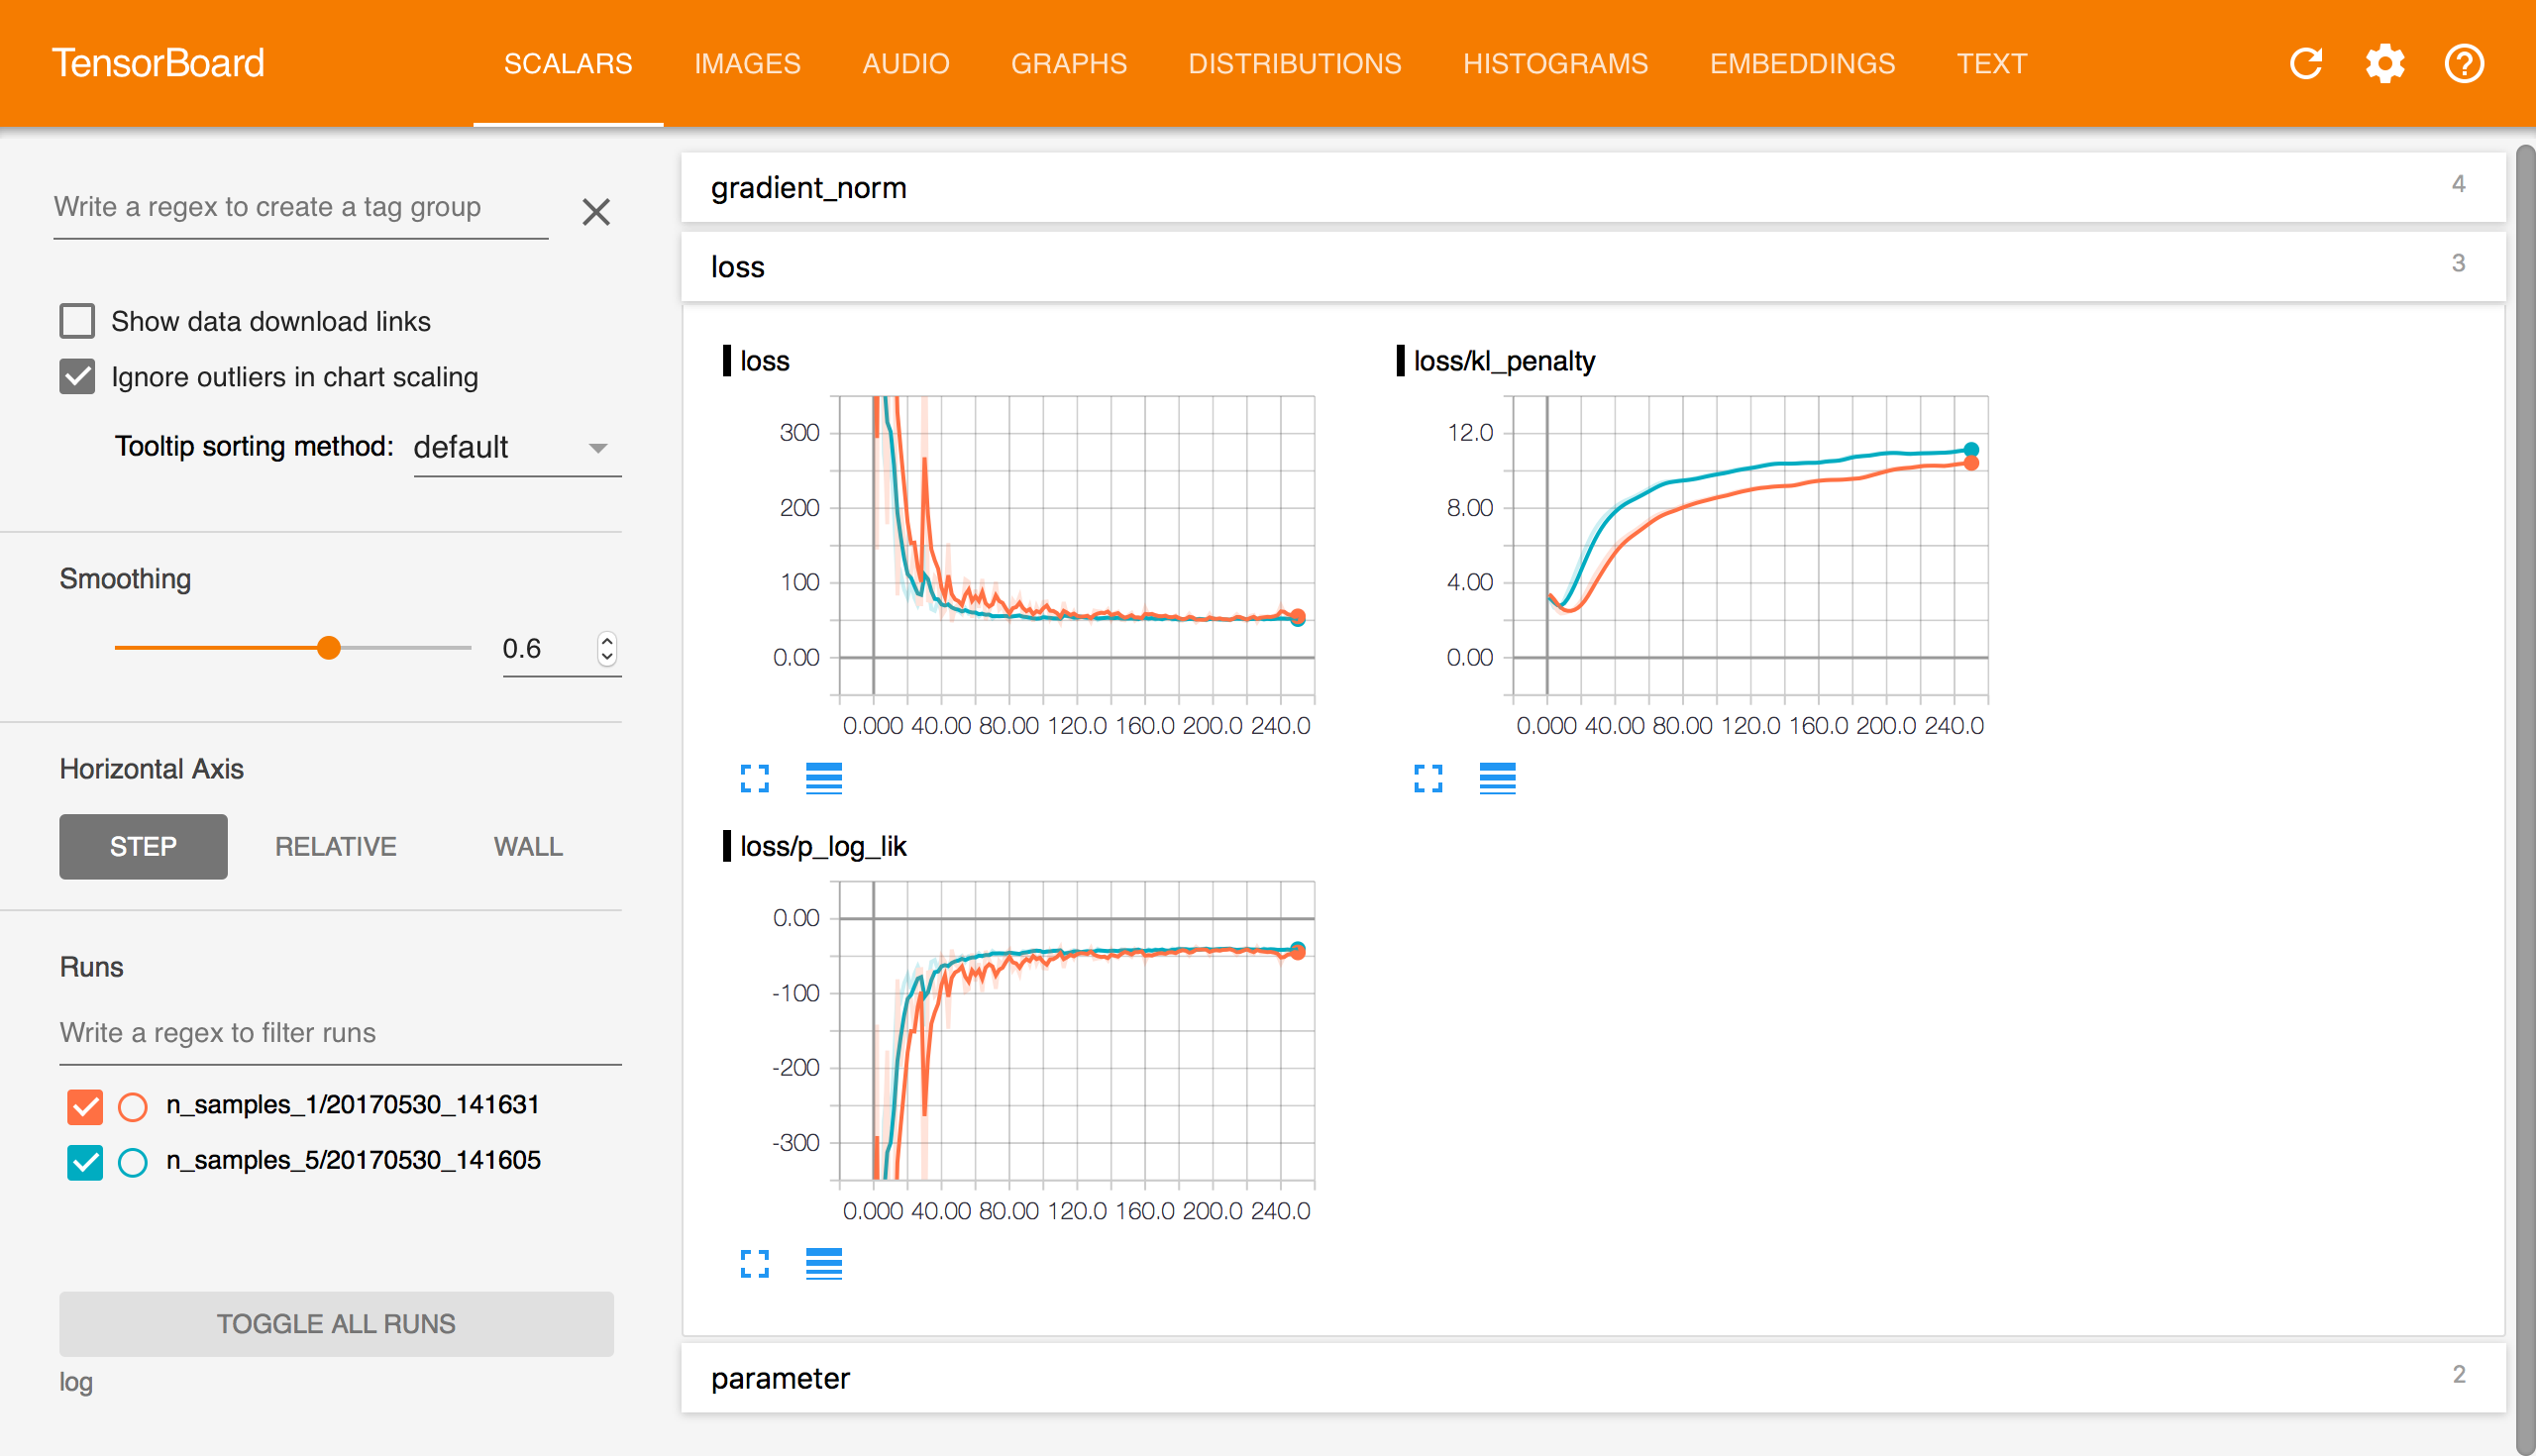
\includegraphics[width=750px]{/images/tensorboard-scalars.png}

To use TensorBoard, we first need to specify a directory for storing
logs during inference. For example, if manually controlling inference,
call

\begin{lstlisting}[language=Python]
inference.initialize(logdir='log')
\end{lstlisting}

If you're using the catch-all \texttt{inference.run()}, include
\texttt{logdir} as an argument. As inference runs, files are
outputted to \texttt{log/} within the working directory. In
commandline, we run TensorBoard and point to that directory.

\begin{lstlisting}[language=JSON]
tensorboard --logdir=log/
\end{lstlisting}

The command will provide a web address to access TensorBoard. By
default, it is \url{http://localhost:6006}. If working correctly, you
should see something like the above picture.

You're set up!

Additional steps need to be taken in order to clean up TensorBoard's
naming. Specifically, we might configure names for random variables
and tensors in the computational graph. To provide a concrete example,
we extend the
\href{http://edwardlib.org/tutorials/supervised-regression}
{supervised learning tutorial},
where the task is to infer hidden structure from labeled examples
$\{(x_n, y_n)\}$.

\subsubsection{Data}

Simulate training and test sets of $40$ data points. They comprise of
pairs of inputs $\mathbf{x}_n\in\mathbb{R}^{5}$ and outputs
$y_n\in\mathbb{R}$. They have a linear dependence with normally
distributed noise.

\begin{lstlisting}[language=Python]
def build_toy_dataset(N, w):
  D = len(w)
  x = np.random.normal(0.0, 2.0, size=(N, D))
  y = np.dot(x, w) + np.random.normal(0.0, 0.01, size=N)
  return x, y

ed.set_seed(42)

N = 40  # number of data points
D = 5  # number of features

w_true = np.random.randn(D) * 0.5
X_train, y_train = build_toy_dataset(N, w_true)
X_test, y_test = build_toy_dataset(N, w_true)
\end{lstlisting}

\subsubsection{Model}

Posit the model as Bayesian linear regression \citep{murphy2012machine}.
For a set of $N$ data points $(\mathbf{X},\mathbf{y})=\{(\mathbf{x}_n, y_n)\}$,
the model posits the following distributions:

\begin{align*}
  p(\mathbf{w})
  &=
  \text{Normal}(\mathbf{w} \mid \mathbf{0}, \sigma_w^2\mathbf{I}),
  \\[1.5ex]
  p(b)
  &=
  \text{Normal}(b \mid 0, \sigma_b^2),
  \\
  p(\mathbf{y} \mid \mathbf{w}, b, \mathbf{X})
  &=
  \prod_{n=1}^N
  \text{Normal}(y_n \mid \mathbf{x}_n^\top\mathbf{w} + b, \sigma_y^2).
\end{align*}

The latent variables are the linear model's weights $\mathbf{w}$ and
intercept $b$, also known as the bias.
Assume $\sigma_w^2,\sigma_b^2$ are known prior variances and $\sigma_y^2$ is a
known likelihood variance. The mean of the likelihood is given by a
linear transformation of the inputs $\mathbf{x}_n$.

Let's build the model in Edward, fixing $\sigma_w,\sigma_b,\sigma_y=1$.

\begin{lstlisting}[language=Python]
with tf.name_scope("model"):
  X = tf.placeholder(tf.float32, [N, D], name="X")
  w = Normal(loc=tf.zeros(D, name="weights/loc"),
             scale=tf.ones(D, name="weights/scale"),
             name="weights")
  b = Normal(loc=tf.zeros(1, name="bias/loc"),
             scale=tf.ones(1, name="bias/scale"),
             name="bias")
  y = Normal(loc=ed.dot(X, w) + b,
             scale=tf.ones(N, name="y/scale"),
             name="y")
\end{lstlisting}

Here, we define a placeholder \texttt{X}. During inference, we pass in
the value for this placeholder according to batches of data.  We also
use a name scope. This adds the scope's name as a prefix
(\texttt{"model/"}) to all tensors in the \texttt{with} context.
Similarly, we name the parameters in each random variable under a
grouped naming system.

\subsubsection{Inference}

We now turn to inferring the posterior using variational inference.
Define the variational model to be a fully factorized normal across
the weights. We add another scope to group naming in the variational
family.

\begin{lstlisting}[language=Python]
with tf.name_scope("posterior"):
  qw = Normal(loc=tf.Variable(tf.random_normal([D]), name="qw/loc"),
              scale=tf.nn.softplus(tf.Variable(tf.random_normal([D]),
                                               name="qw/unconstrained_scale")),
              name="qw")
  qb = Normal(loc=tf.Variable(tf.random_normal([1]), name="qb/loc"),
              scale=tf.nn.softplus(tf.Variable(tf.random_normal([1]),
                                               name="qb/unconstrained_scale")),
              name="qb")
\end{lstlisting}

Run variational inference with the Kullback-Leibler divergence.
We use $5$ latent variable samples for computing
black box stochastic gradients in the algorithm.
(For more details, see the
\href{/tutorials/klqp}{$\text{KL}(q\|p)$ tutorial}.)

\begin{lstlisting}[language=Python]
inference = ed.KLqp({w: qw, b: qb}, data={X: X_train, y: y_train})
inference.run(n_samples=5, n_iter=250, logdir='log/n_samples_5')
\end{lstlisting}

\begin{lstlisting}
250/250 [100%] ██████████████████████████████ Elapsed: 5s | Loss: 50.865
\end{lstlisting}

Optionally, we might include an \texttt{"inference"} name scope.
If it is absent, the charts are partitioned naturally
and not automatically grouped under the monolithic \texttt{"inference"}.
If it is added, the computational graph is slightly more organized.

\subsubsection{Criticism}

We can use TensorBoard to explore learning and diagnose any problems.
After running TensorBoard with the command above, we can navigate the
tabs.

Below we assume the above code is run twice with different
configurations
of the \texttt{n_samples} hyperparameter.
We specified the log directory to be \texttt{log/n_samples_*}.
By default, Edward also includes a timestamped subdirectory so that
multiple runs of the same experiment have properly organized logs for
TensorBoard. You can turn it off by specifying
\texttt{log_timestamp=False} during inference.

\textbf{TensorBoard Scalars.}

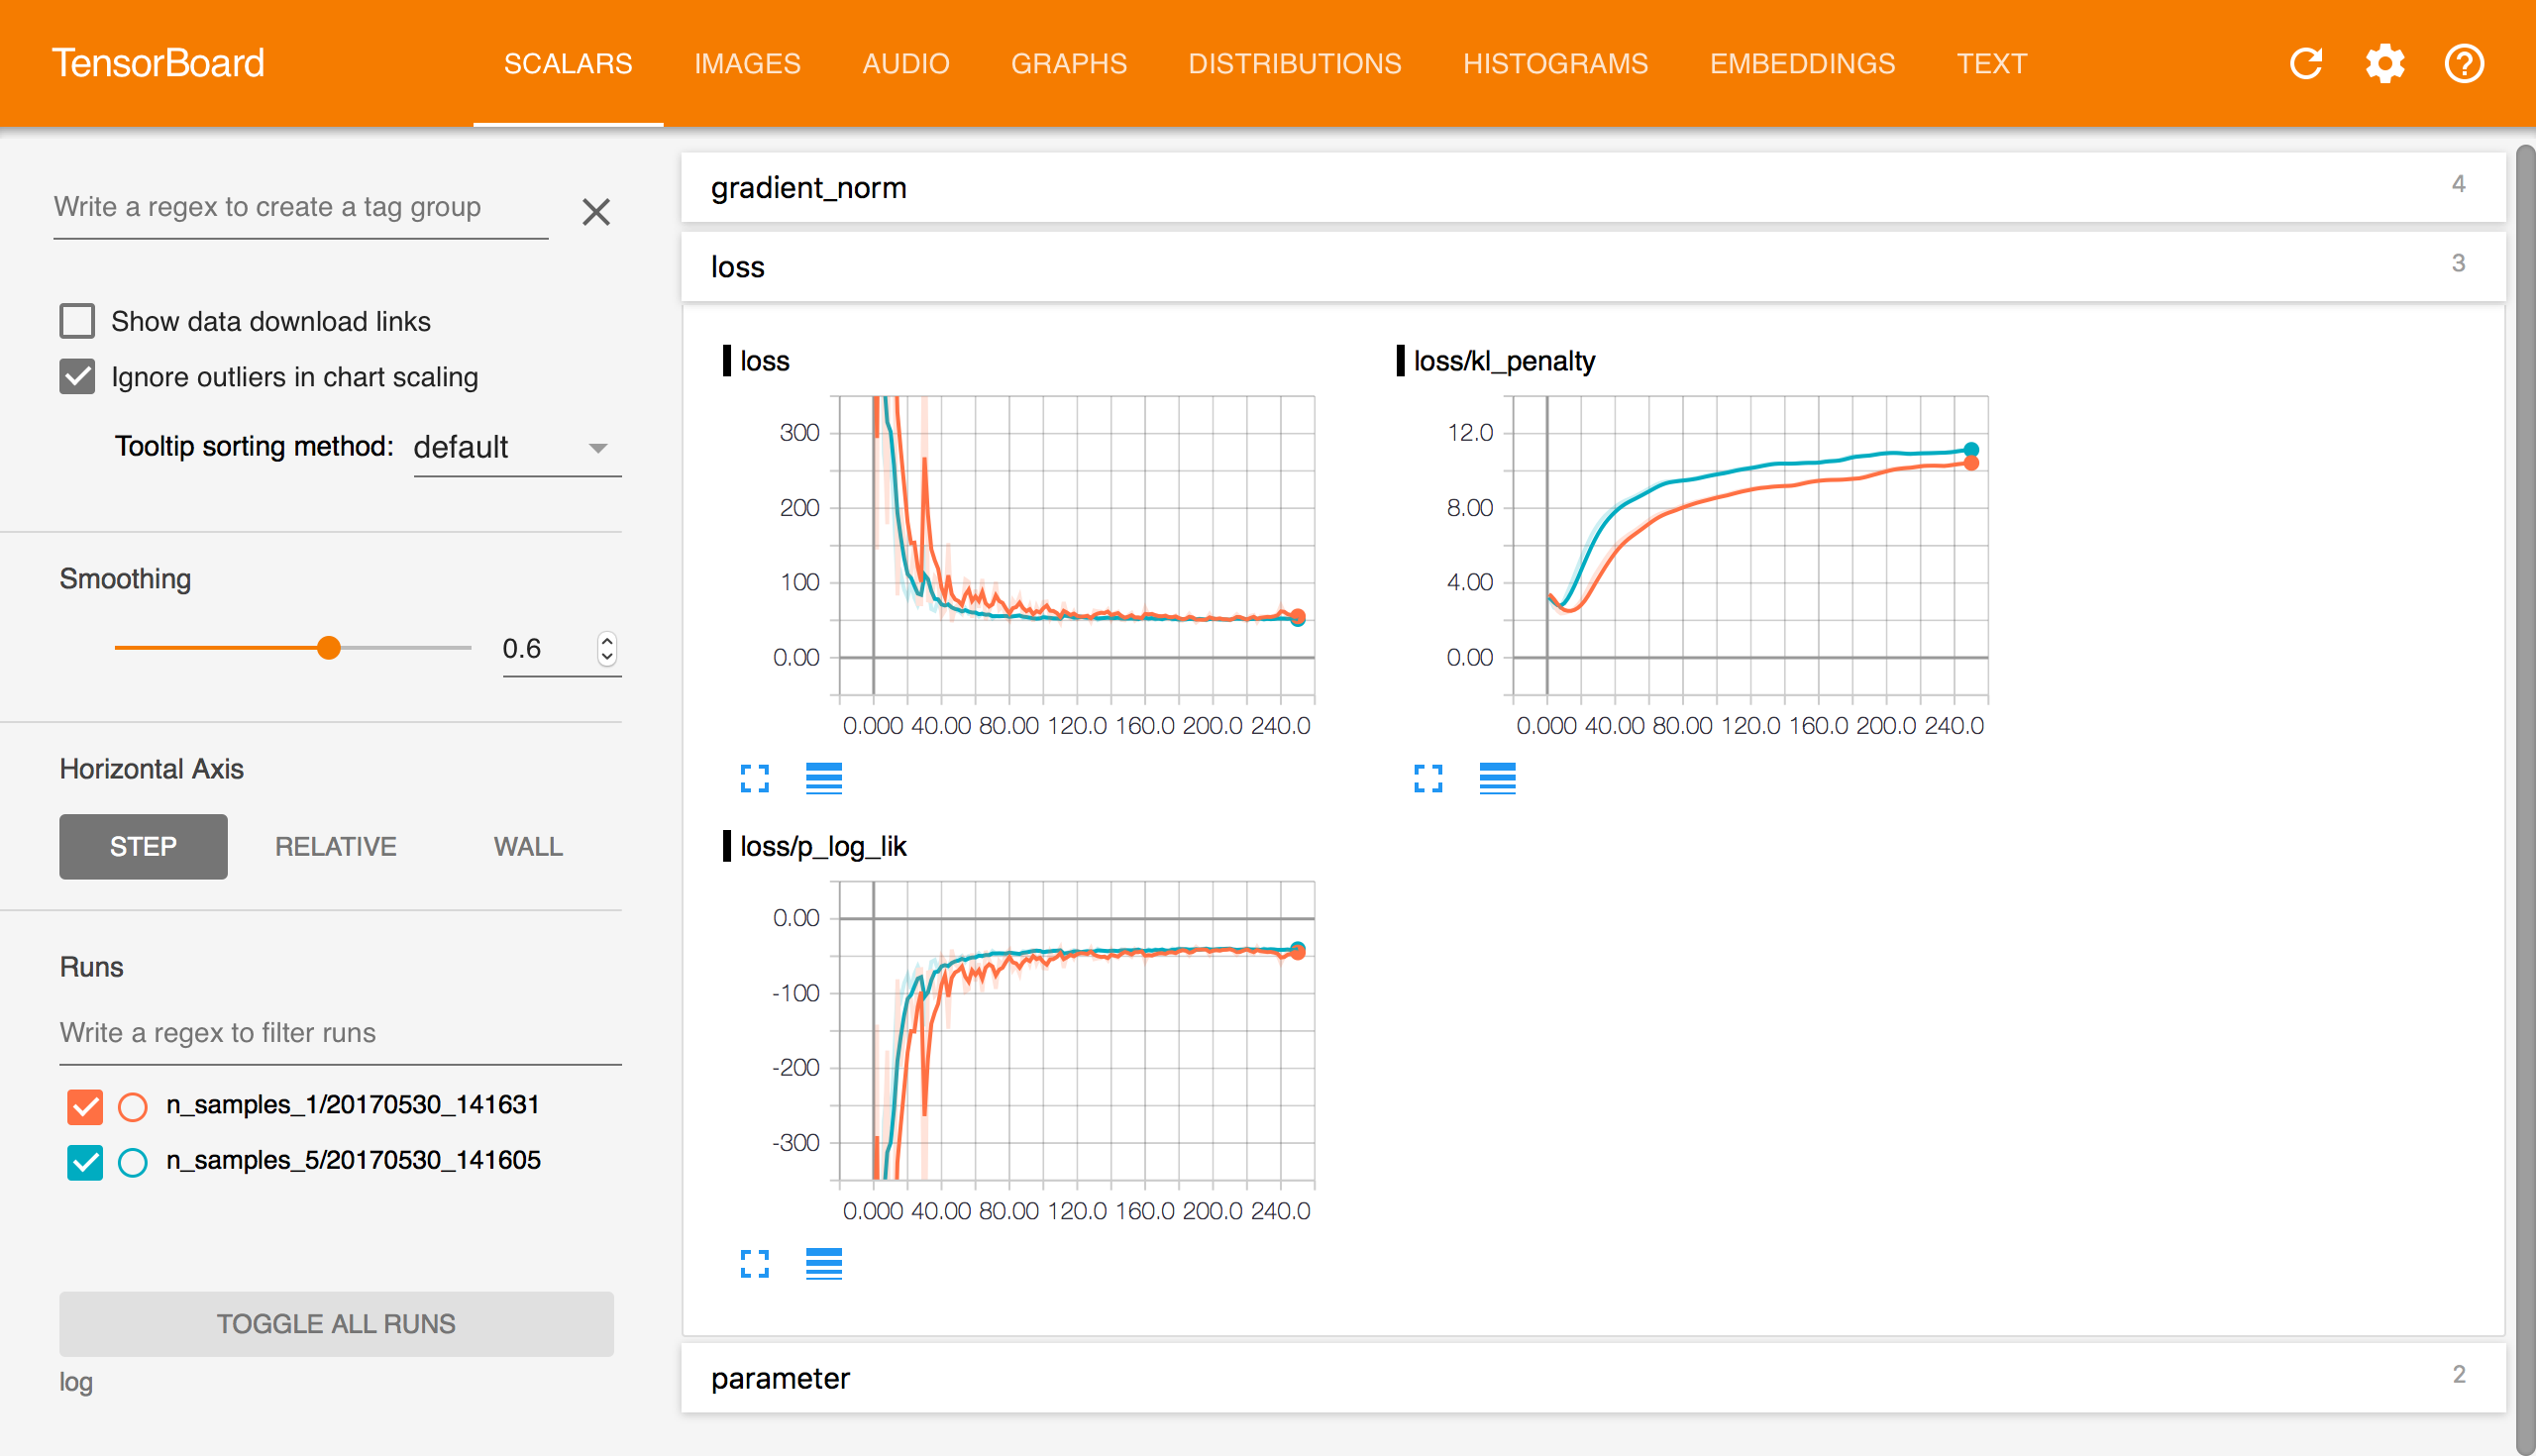
\includegraphics[width=750px]{/images/tensorboard-scalars.png}

Scalars provides scalar-valued information across iterations of the
algorithm, wall time, and relative wall time. In Edward, the tab
includes the value of scalar TensorFlow variables (free parameters) in
the model or approximating family.

With variational inference, we also include information such as the
loss function and its decomposition into individual terms. This
particular example shows that \texttt{n_samples=1} tends to have higher
variance than \texttt{n_samples=5} but still converges to the same solution.

\textbf{TensorBoard Graphs.}

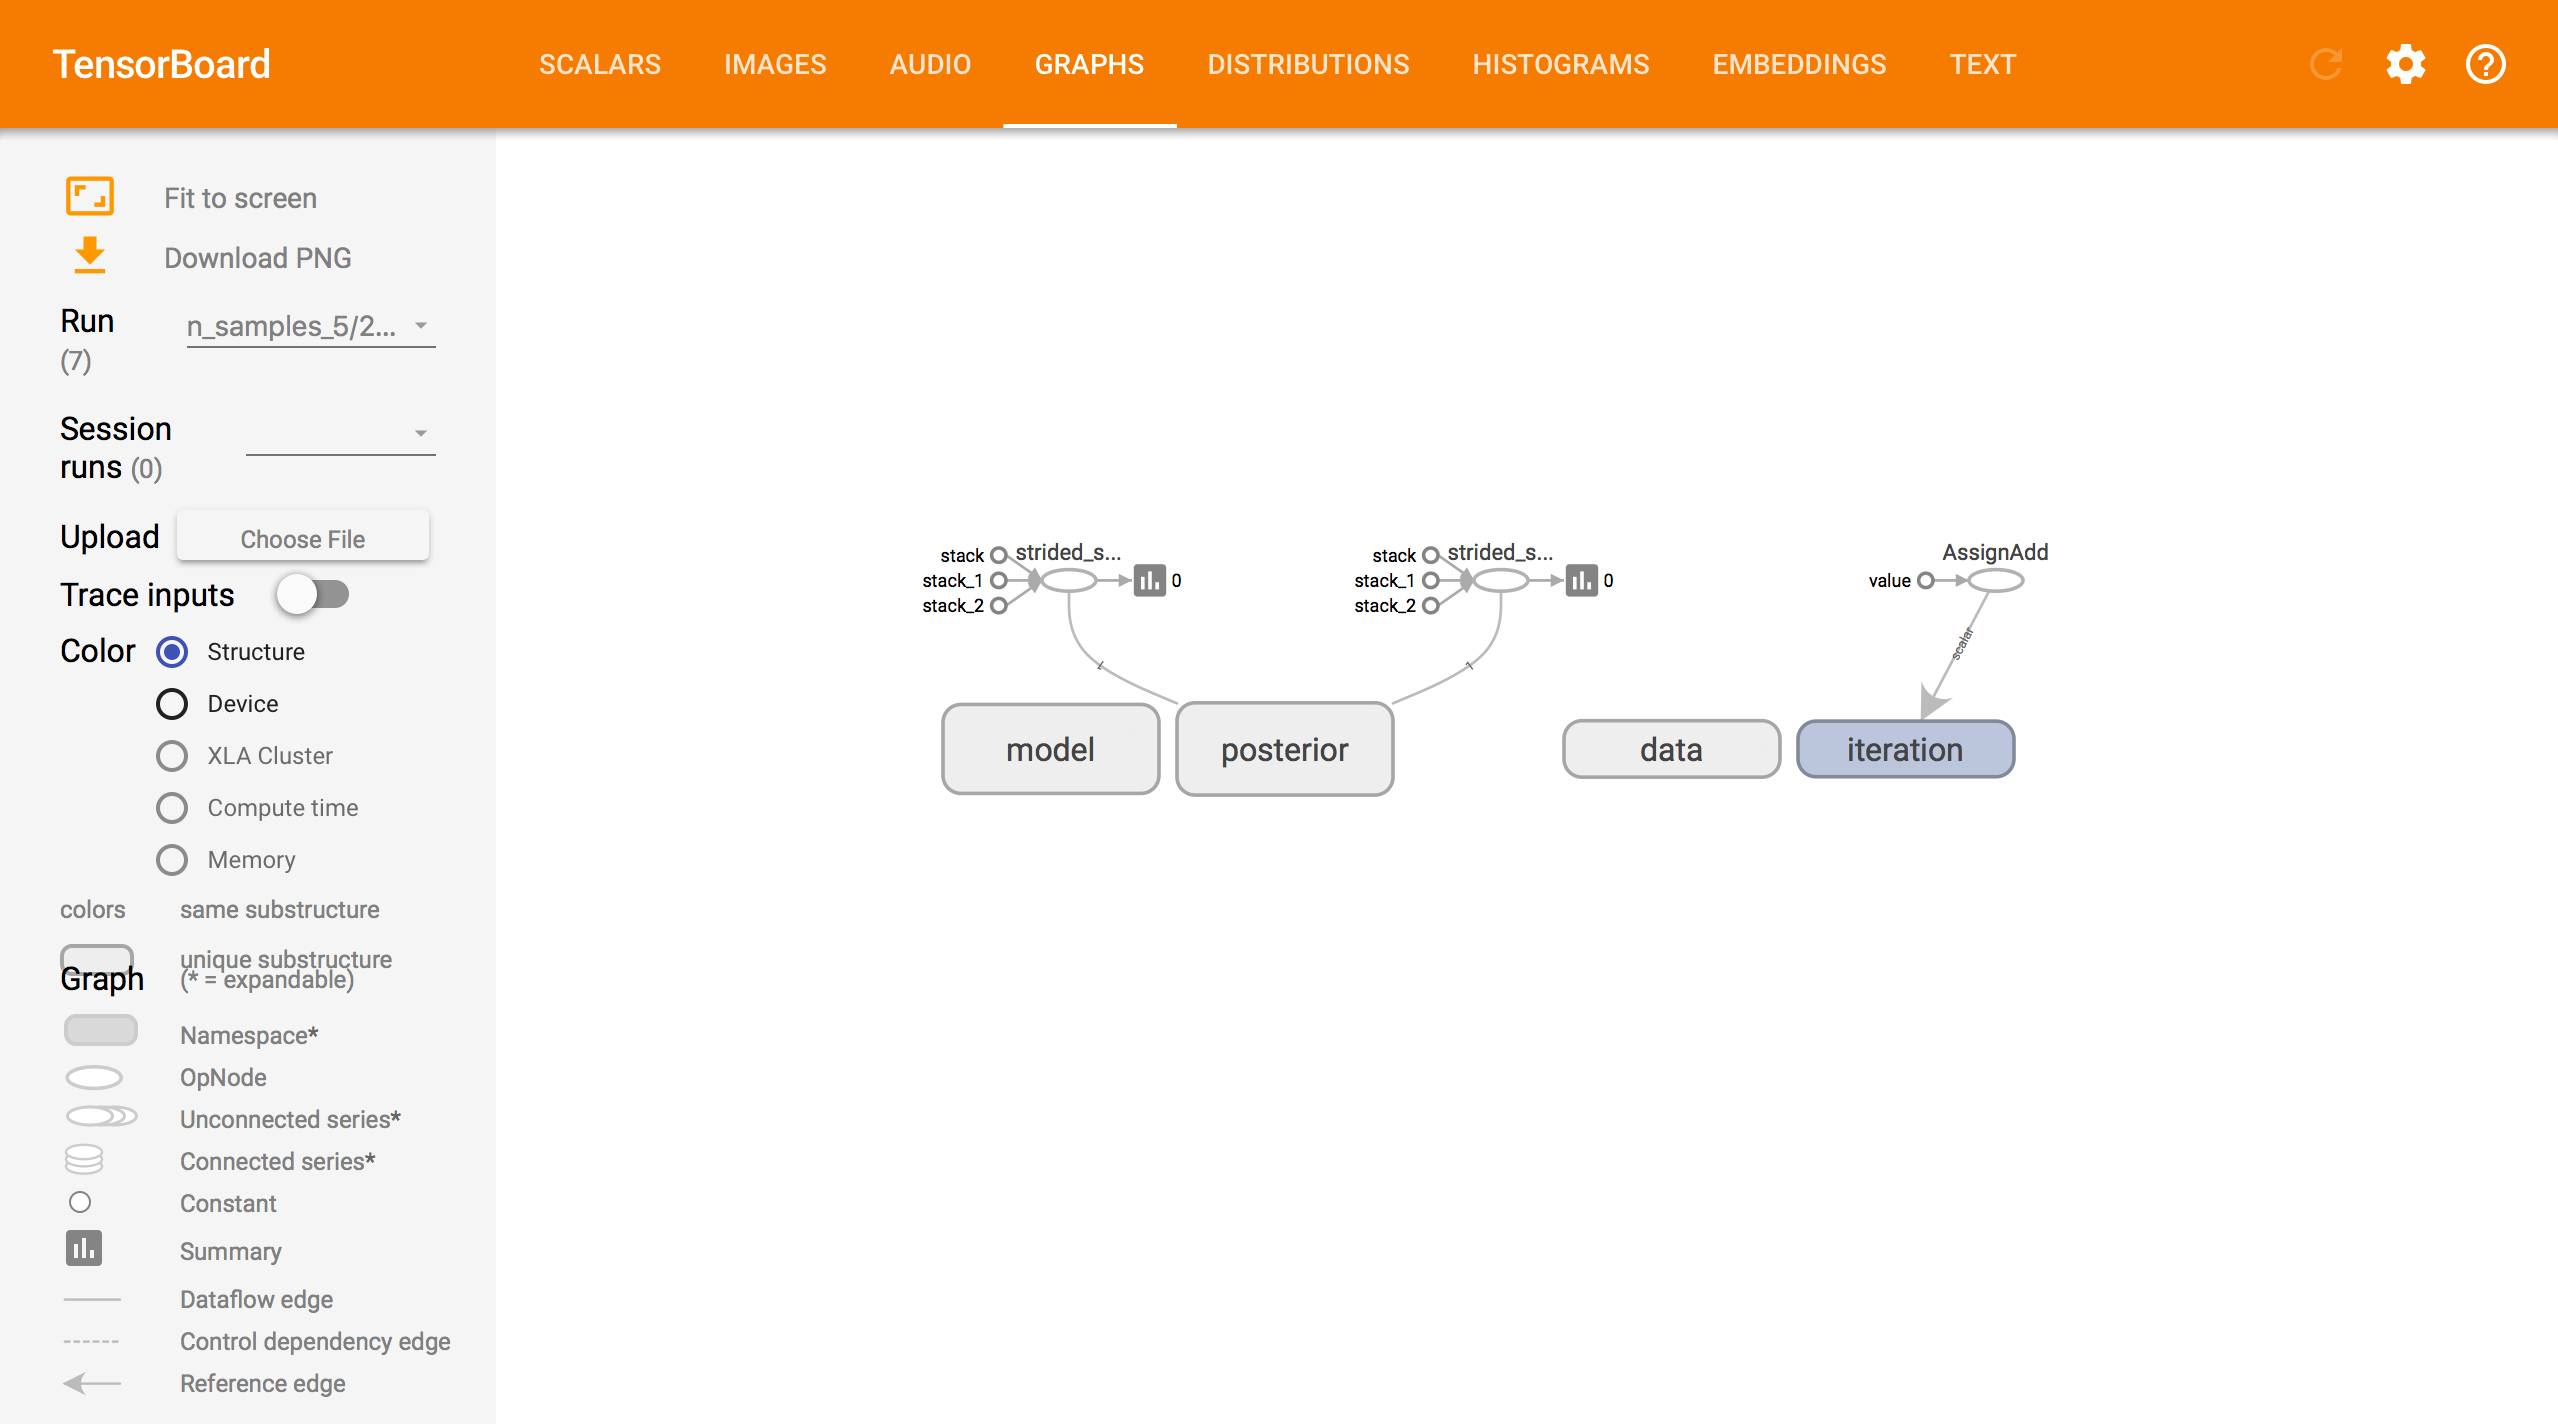
\includegraphics[width=750px]{/images/tensorboard-graphs-0.png} \\
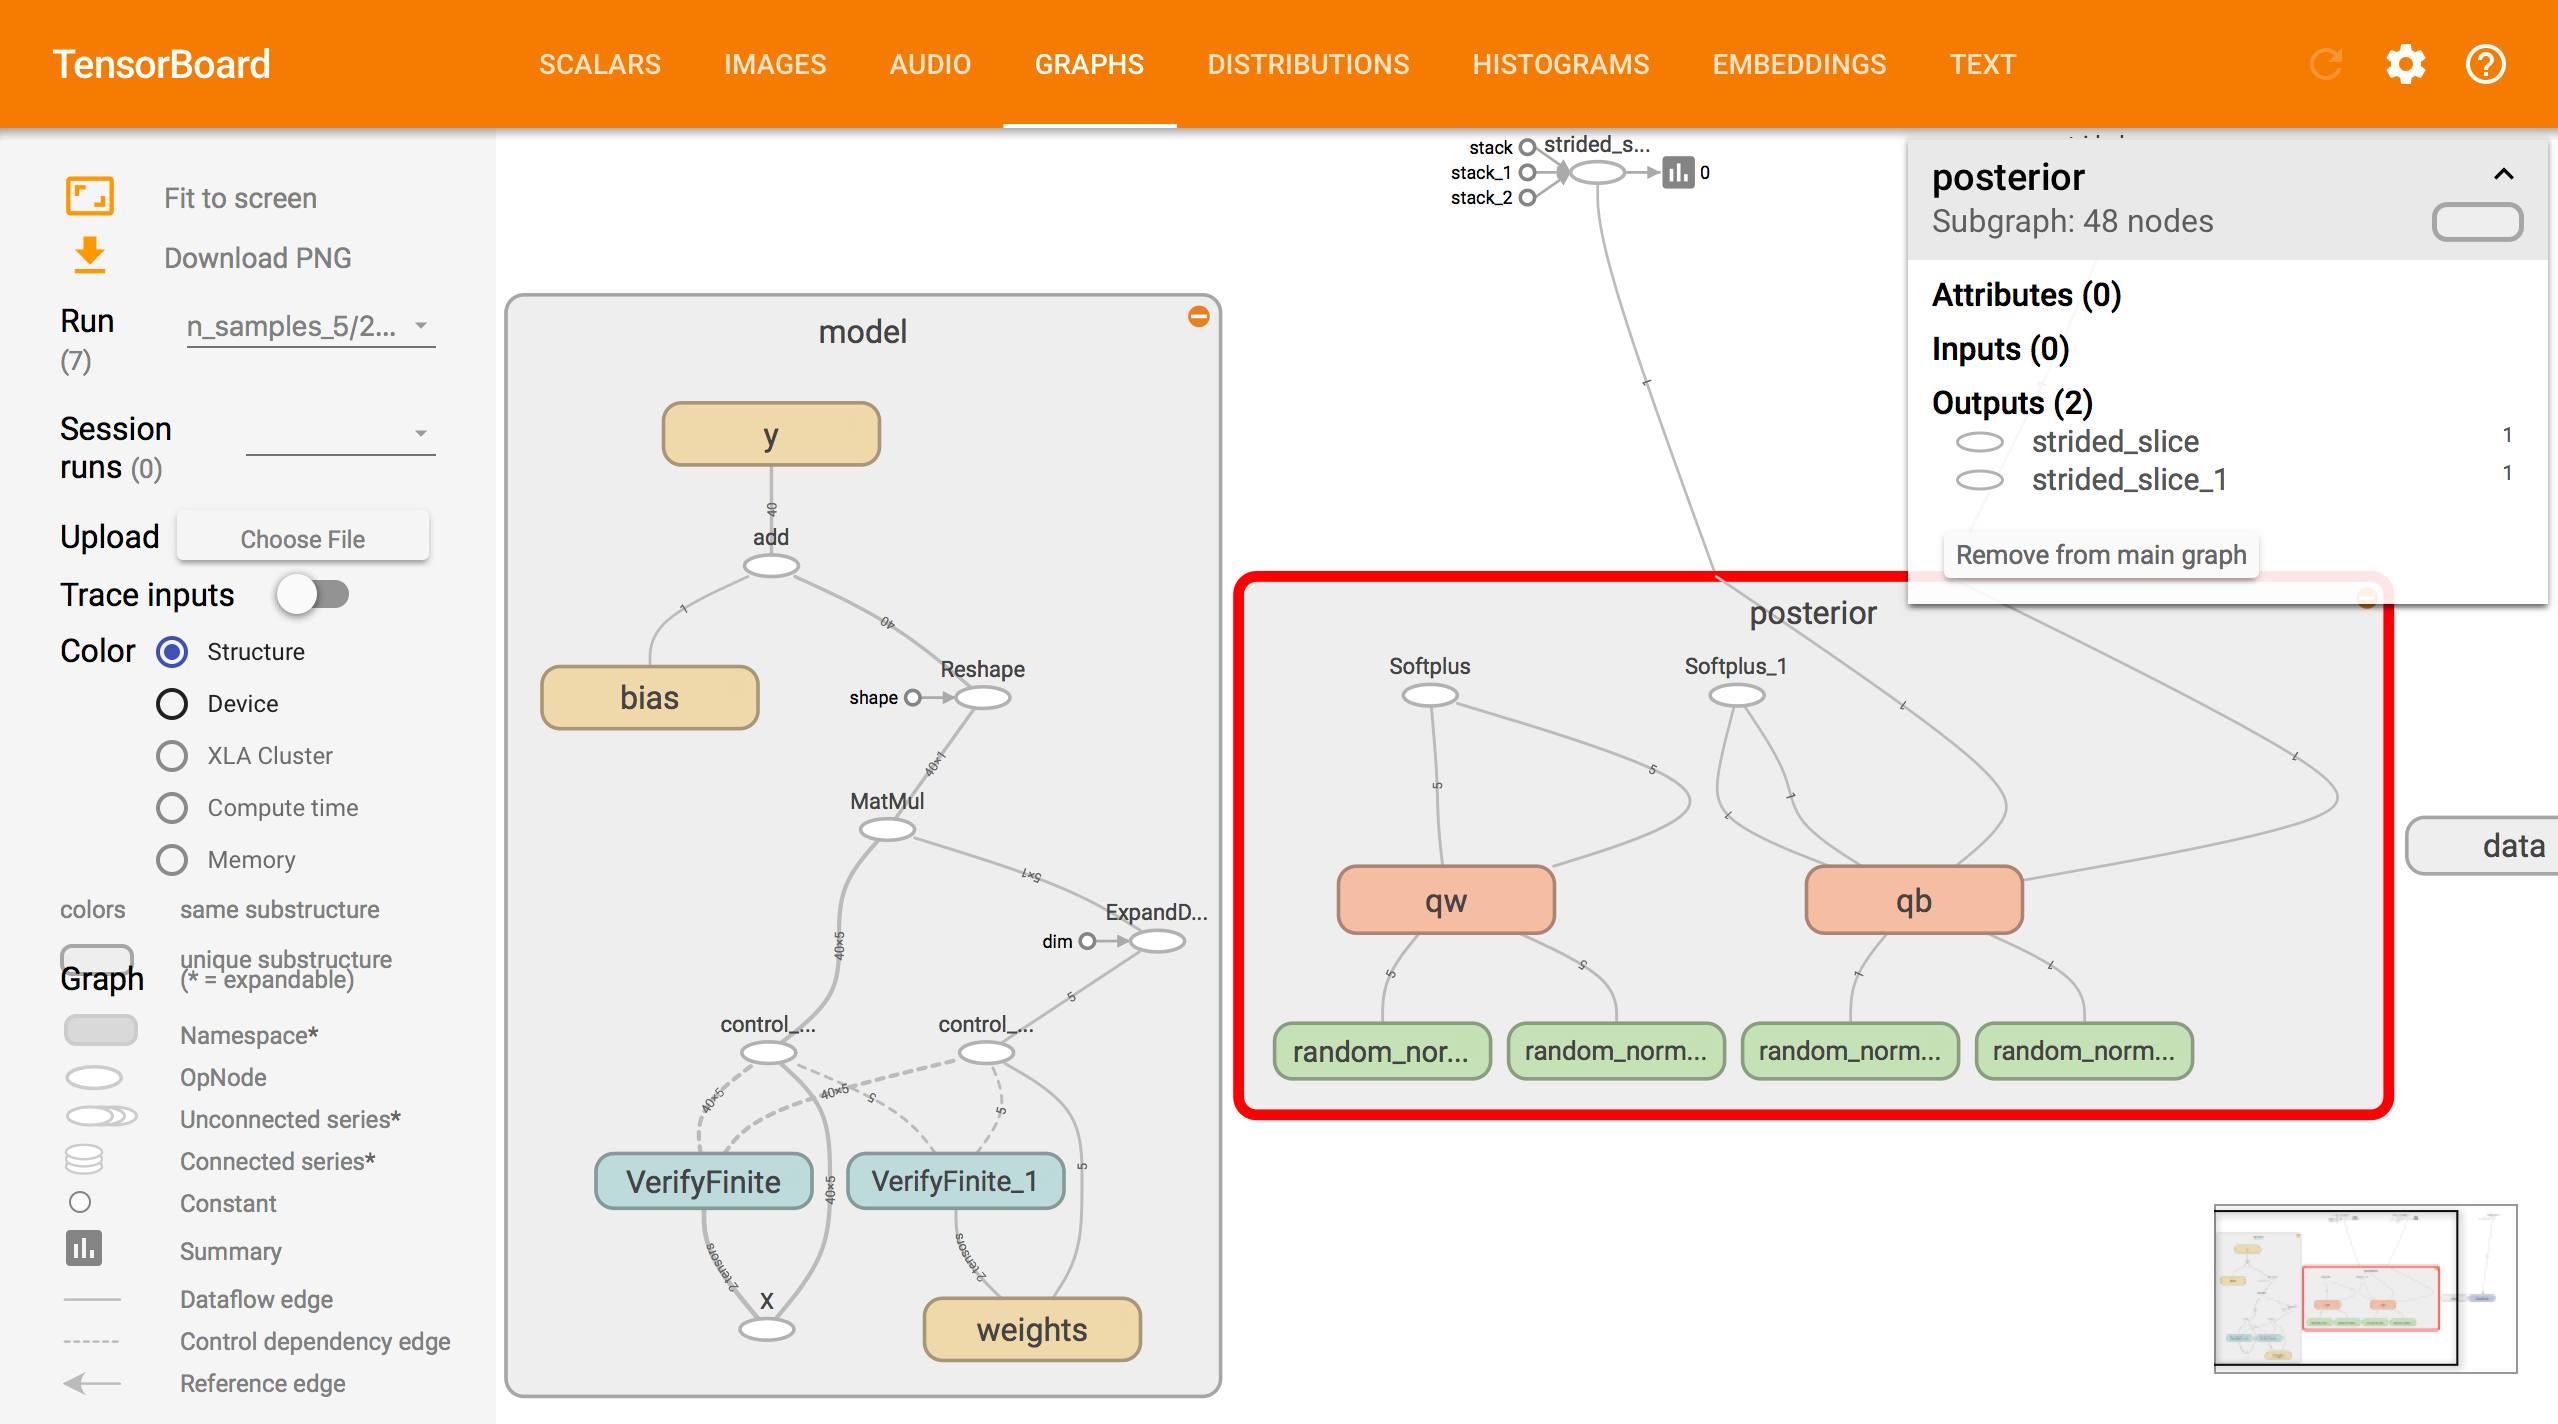
\includegraphics[width=750px]{/images/tensorboard-graphs-1.png}

Graphs displays the computational graph underlying the model,
approximating family, and inference. Boxes denote tensors grouped
under the same name scope. Cleaning up names in the graph makes it
easy to better understand and optimize your code.

\textbf{TensorBoard Distributions.}

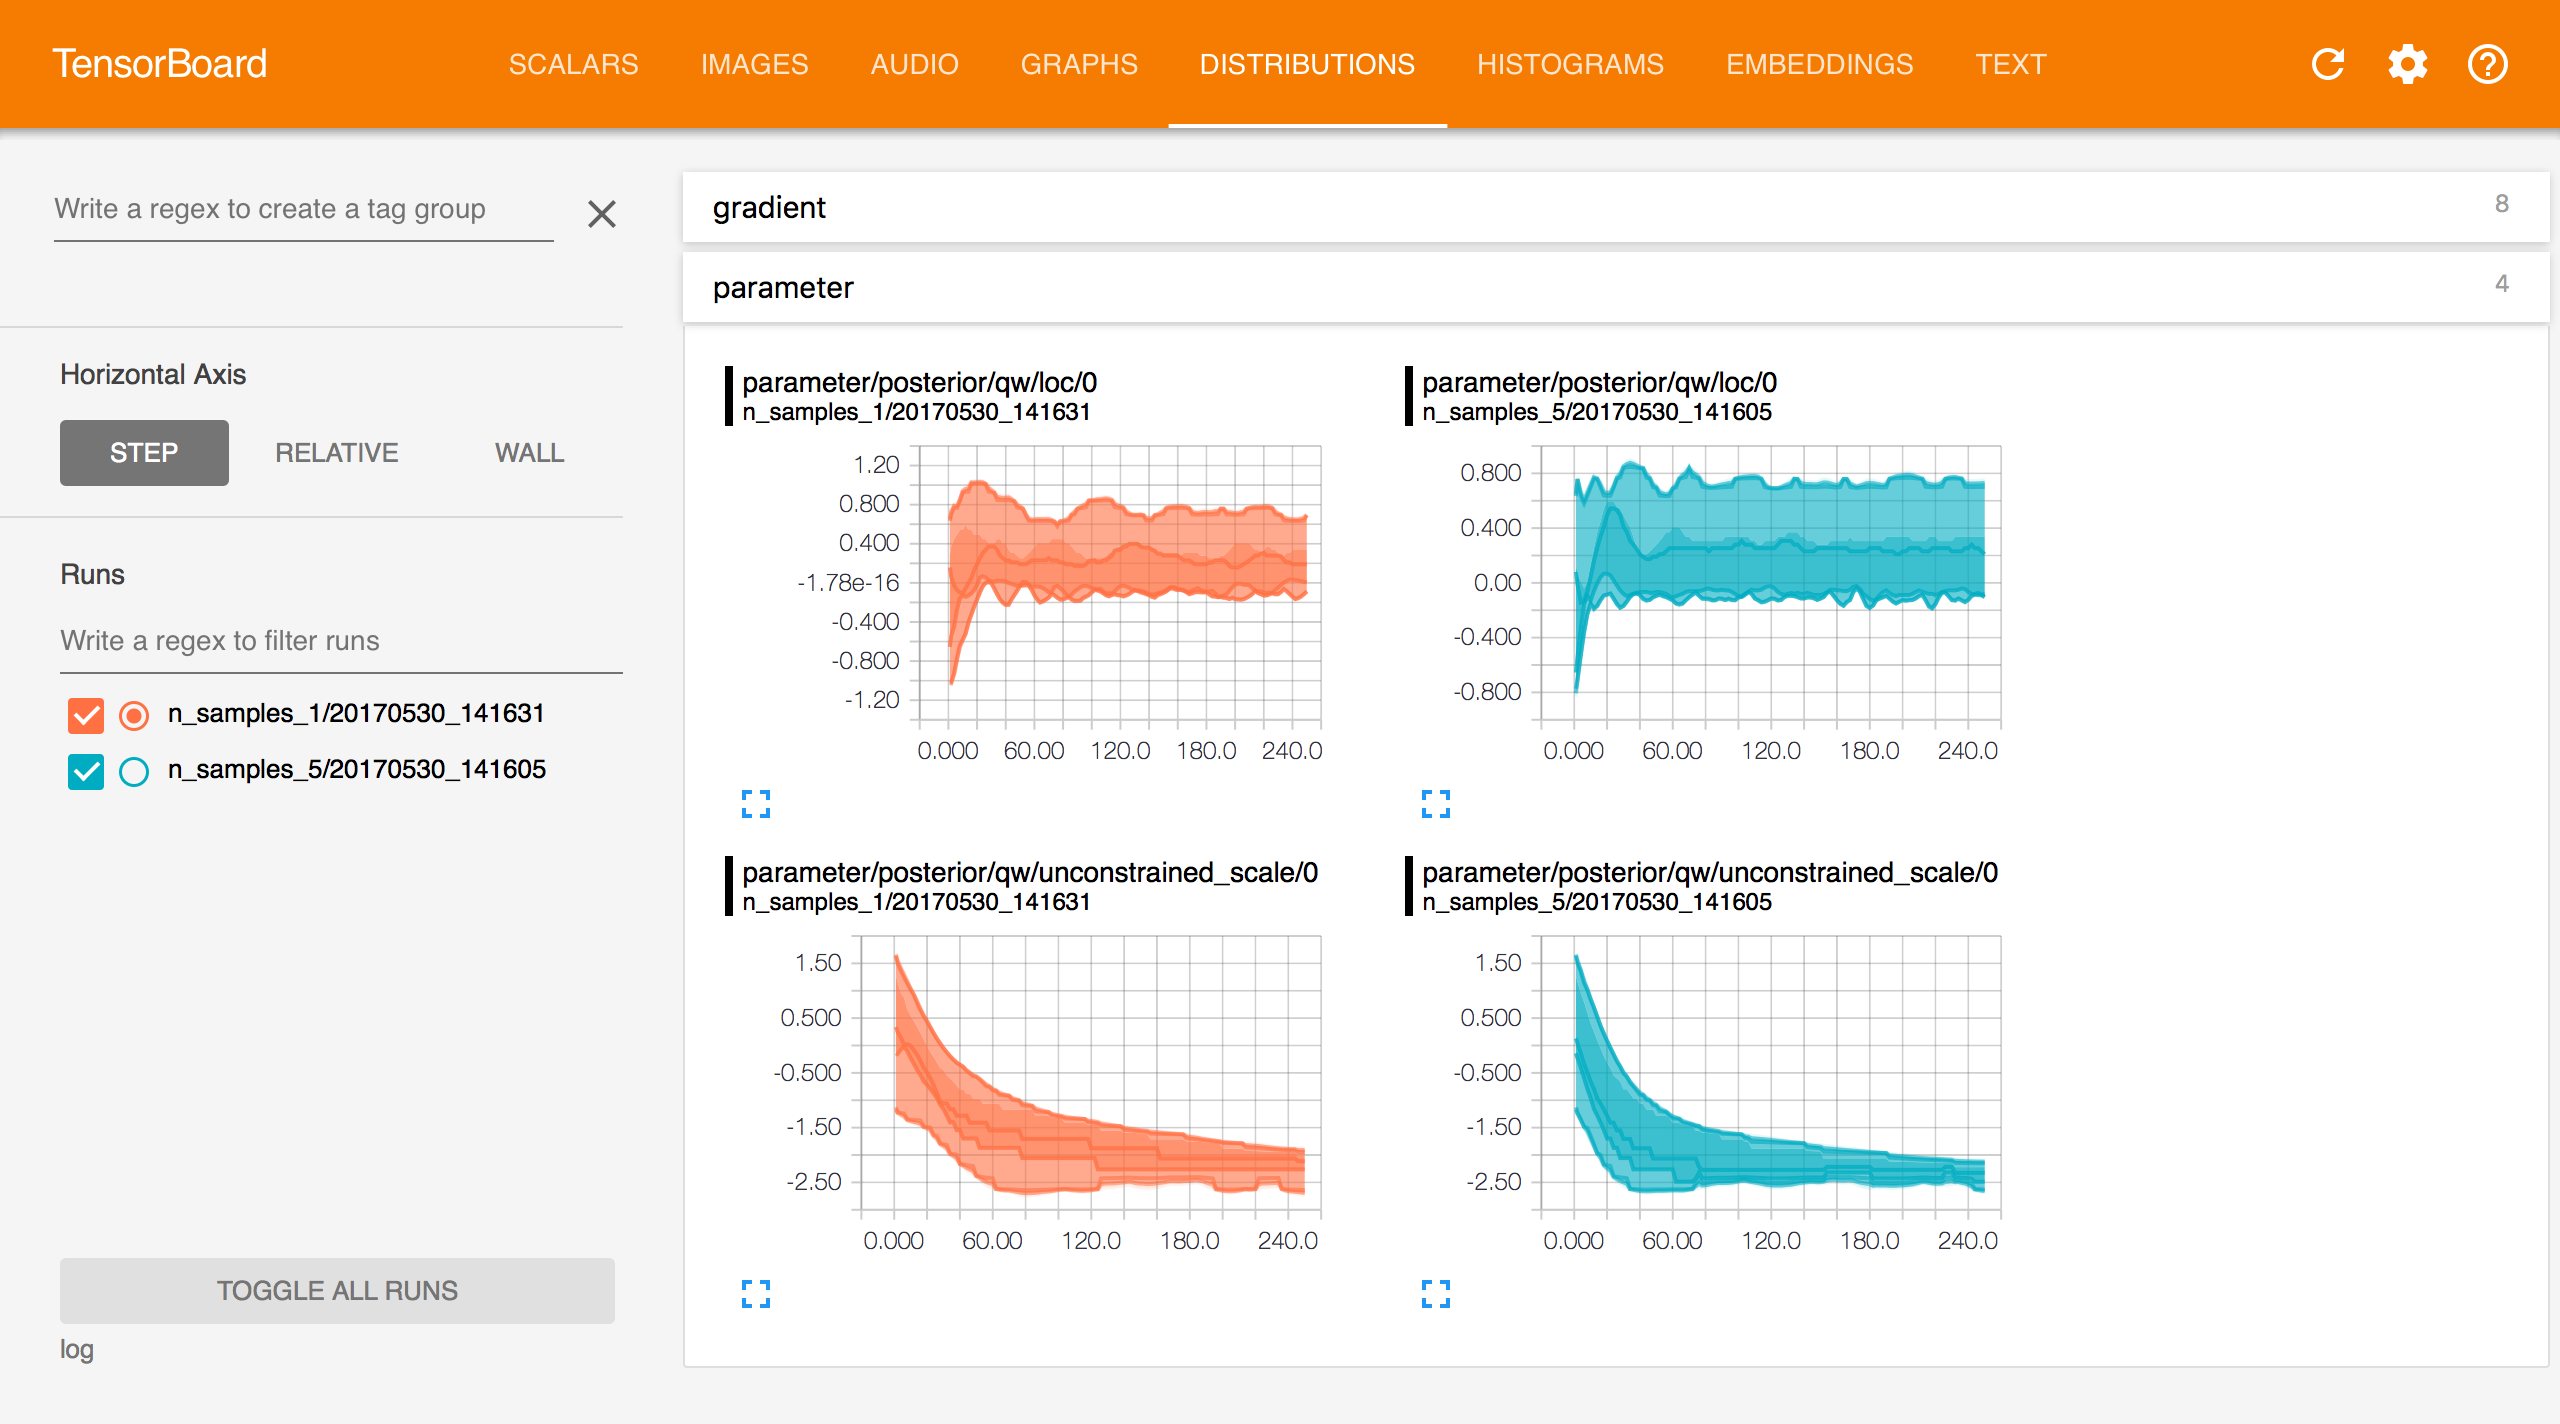
\includegraphics[width=750px]{/images/tensorboard-distributions.png}

Distributions displays the distribution of each non-scalar TensorFlow
variable across iterations. These variables are the free parameters
of your model and approximating family.

\textbf{TensorBoard Histograms.}

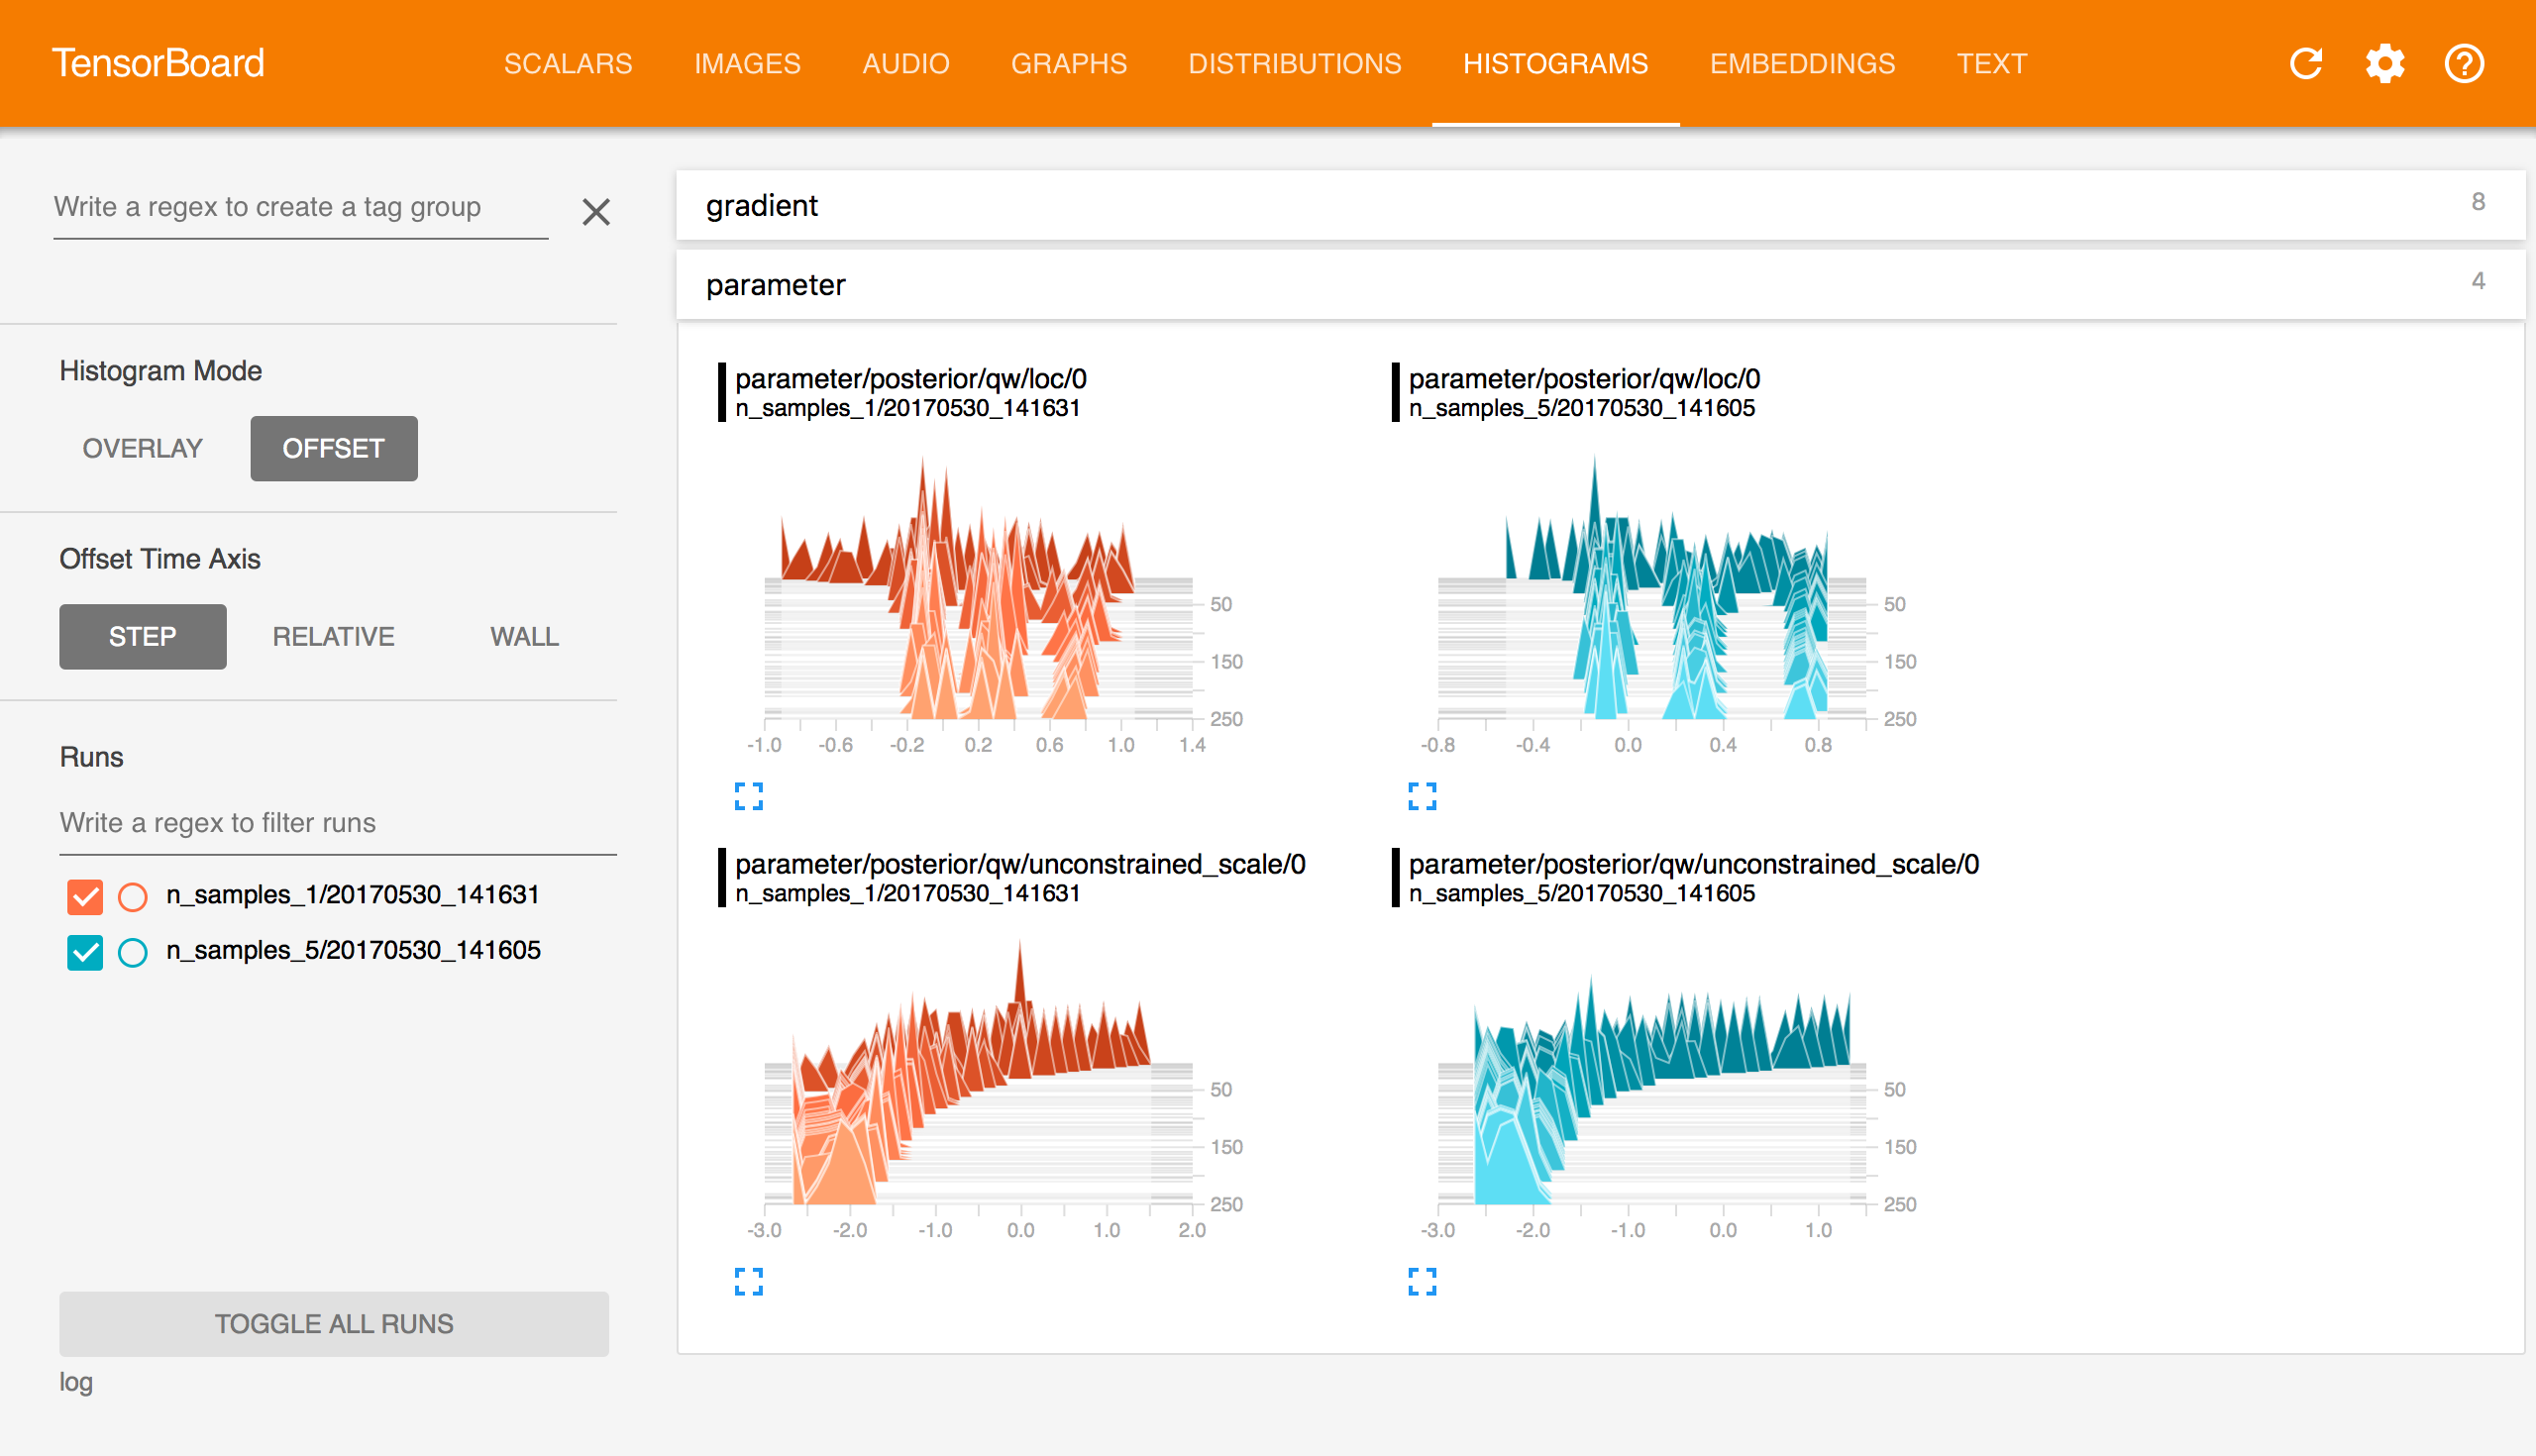
\includegraphics[width=750px]{/images/tensorboard-histograms.png}

Histograms displays the same information as Distributions but as a 3-D
histogram changing aross iteration.

\subsubsection{Acknowledgments}

We thank Sean Kruzel for writing the initial version of this
tutorial.

A TensorFlow tutorial to TensorBoard can be found
\href{https://www.tensorflow.org/get_started/summaries_and_tensorboard}
{here}.

\subsubsection{References}\label{references}
